\documentclass[tikz,border=10pt]{standalone}
\usepackage{tikz}
\usetikzlibrary{positioning}

\definecolor{blobred}{RGB}{140,20,20} % nice dark red

\begin{document}
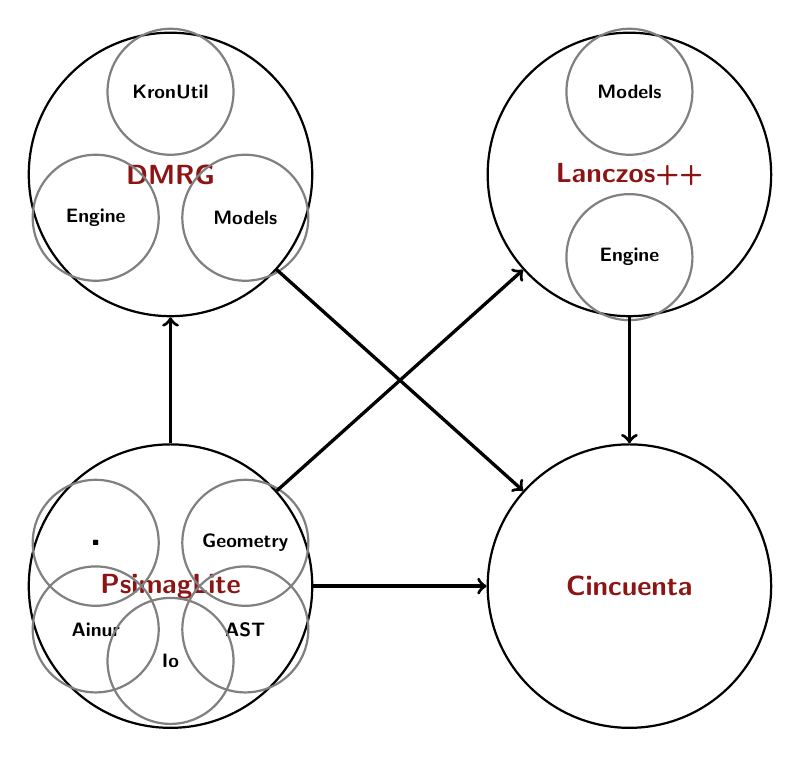
\begin{tikzpicture}[
  blob/.style={
    draw,
    circle,
    thick,
    align=center,
    font=\sffamily\bfseries\color{blobred},
    minimum width=3.6cm,
    minimum height=1.8cm
  },
  subblob/.style={
    draw=gray,
    circle,
    thick,
    align=center,
    font=\sffamily\scriptsize\bfseries, % not red
    minimum width=1.6cm,
    minimum height=0.8cm,
    inner sep=2pt
  },
  arr/.style={->, very thick}
]
\node[blob] (dmrg) {DMRG};
\node[blob, right=2.2cm of dmrg] (lanczos) {Lanczos++};
\node[blob, below=1.6cm of dmrg] (psimag) {PsimagLite};
\node[blob, right=2.2cm of psimag] (cincuenta) {Cincuenta};

% Sub-blobs inside DMRG
\node[subblob] at ([xshift=-0.95cm,yshift=-0.55cm]dmrg.center) {Engine};
\node[subblob] at ([xshift=0.95cm,yshift=-0.55cm]dmrg.center)  {Models};
\node[subblob] at ([xshift=0.00cm,yshift=1.05cm]dmrg.center)   {KronUtil};

% Sub-blobs inside Lanczos++
\node[subblob] at ([xshift=0.0cm,yshift=-1.05cm]lanczos.center) {Engine};
\node[subblob] at ([xshift=0.0cm,yshift=1.05cm]lanczos.center)  {Models};

% Sub-blobs inside PsimagLite
	\node[subblob] at ([xshift=-0.95cm,yshift=0.55cm]psimag.center) {{\Large .}};
\node[subblob] at ([xshift=0.95cm,yshift=0.55cm]psimag.center)  {Geometry};
\node[subblob] at ([xshift=-0.95cm,yshift=-0.55cm]psimag.center) {Ainur};
\node[subblob] at ([xshift=0.95cm,yshift=-0.55cm]psimag.center)  {AST};
	\node[subblob] at ([xshift=0.0, yshift=-0.95cm]psimag.center) {Io};
% Arrows
\draw[arr] (psimag) -- (dmrg);
\draw[arr] (psimag) -- (lanczos);
\draw[arr] (psimag) -- (cincuenta);
\draw[arr] (dmrg) -- (cincuenta);
\draw[arr] (lanczos) -- (cincuenta);

\end{tikzpicture}
\end{document}

